\chapter{Evaluations and Results}
\markright{Aravindan Mahendiran \hfill Chapter 4. Evaluations and Results \hfill}
To evaluate our hypothesis about the vocabularies we test our models on eight different presidential elections from Latin America using both the seed vocabulary and the vocabulary generated by the query expansion algorithm.
We use the results obtained using the seed vocabulary detailed in the previous section as a baseline score.
We then use the same vocabulary to seed our PSL learning algorithm. 
The prediction algorithms are then run again, now by using the expanded vocabulary obtained through the query expansion.
In order to remain consistent with predicting ahead of time, we track only the hashtags identified by the query expansion pipeline  until that particular date.

\begin{figure*}
	\centering
	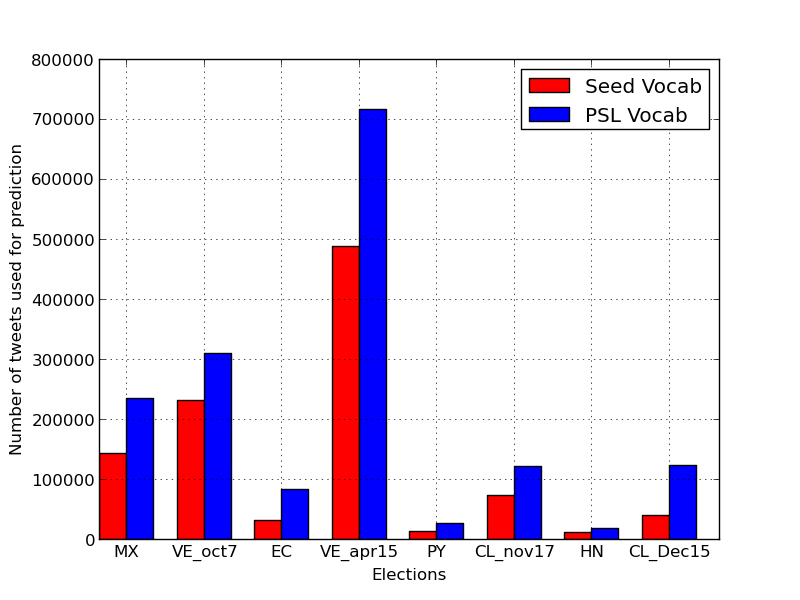
\includegraphics[scale=0.65]{support_files/Recall.png}
	\caption{Recall of seed vocabulary vs PSL vocabulary}
	\label{fig:recall}
\end{figure*}

Figure \ref{fig:recall} shows the increase in the number of documents that were used by the algorithms to make a predictions.
It is noticed when averaged across all the eight elections we notice close to a two-fold increase in the number of 
tweets that were used by these models.
This is a substantial increase of relevant tweets for the domain.

\begin{table*}
	\centering
	\begin{tabular}{| l || r | r | r | r | r | r |}
 	\hline
 	Election & UniVis+Seed & UniVis+PSL & Improvement & Reg+Seed & Reg+PSL & Improvement\\
 	\hline
	Mexico & 0.353 & 0.368 & -4.2\% & 0.123 & 0.07 & 43.09\% \\ 	
 	Venezuela\_Oct7 & 0.069	& 0.077 & -11.59\% & 0.158 & 0.109 & 31.01\&\\
	Ecuador & 0.531 & 0.547 & -3.01\% & 0.263 & 0.244 & 7.22\% \\
	Venezuela\_Apr15 & 0.198 & 0.178 & 10.10\% & 0.142 & 0.112 & 21.126\&\\
	Paraguay & 0.34 & 0.288 & 15.29\% & 0.2 & 0.18 & 10\% \\
	Chile\_Nov17 & 0.56 & 0.42 & 25\% & 0.245 & 0.207 & 15.51\% \\
	Honduras & 0.563 & 0.527 & 6.39\% & 0.293 & 0.184 & 37.20\% \\
	Chile\_Dec17 & 0.096 & 0.061 & 36.45\% & 0.409 & 0.369 & 9.77\% \\
 	\hline
	\end{tabular}
	\caption{Improvement in prediction accuracy}
	\label{table:improvement}
\end{table*}	

To further illustrate the fact that the vocabulary used by such algorithms plays a vital role, we compare the performance of the models using the two different vocabularies.
The Mean Absolute Percentage Error (MAPE) was used as a metric to measure the performance of the models. 
To reduce the effect of outliers we track the popularity of only the major candidates and ignore the ones who obtained less than 10\% of the total votes.


Table \ref{table:improvement} shows the performance of each vocabulary in different elections. 
On an average it is seen that the mean absolute percentage error is reduced by 15.58\%.
We see greater and more consistent improvement with the regression model as the model weighs each window of tweets differently depending upon the opinion poll time series whereas the unique visitor model values them equally. 
Therefore, when the algorithm uses the `not-so-informative' hashtags identified during 
the earlier iterations, the sentiment value and the counts of these mentions bring down the accuracy of the model even though at a later stage hash-tags that are strongly indicative of a user's preference is picked up.
So words such as "facebook" which occur commonly dominate the counts and therefore skew the results even though they are dropped from the vocabulary at a later point.
